
%%%%    IMPORTS 2 BASE    %%%%


\documentclass[hidelinks, french, oneside]{article}
\usepackage[utf8]{inputenc}
\usepackage[T1]{fontenc}

% pour le mise en page
\usepackage[a4paper, total={6.5in, 10in}]{geometry}
\usepackage{fontsize} \changefontsize[13]{10}		
\usepackage{xcolor}

% mathsymbole
\usepackage{amsmath, amssymb,stmaryrd}
\usepackage{wasysym}[mathcal] % a quoi sert le [mathcal] ?
\usepackage{nicefrac, units} % fraction pour text mode / unité

% TBD
\usepackage{mathcomp}
\usepackage{mathrsfs} % pour \mathscr a priori

% pour les belles fonts
\usepackage{amsfonts}
\DeclareMathAlphabet{\mathpzc}{OT1}{pzc}{m}{it}
%\usepackage{euscript}[mathcal]
%\usepackage{rsfso}
\usepackage{bbm}	 % mathbb étendu

% pour les hyprlien / cross-ref
\usepackage{hyperref, cleveref}
%\namecref{sec:label}

%pour les figures
\usepackage{graphicx} \usepackage{wrapfig, floatrow}
%\usepackage{subcaption} % surement useless, parsk floatrow-like 

% pour les beaux tableaux
\usepackage{multirow}

% pour des matrices infernales
\usepackage{easybmat}

% pour les citations (aucune idées de comment ca marche)
\usepackage{csquotes}



%%%%    RACCOURCIS    %%%%


% bb / cal / frak
\newcommand{\N}{\mathbb{N}}
\newcommand{\Z}{\mathbb{Z}}             % Note pour homo pour les updates
\newcommand{\Q}{\mathbb{Q}}
\newcommand{\R}{\mathbb{R}}
\newcommand{\C}{\mathbb{C}}
\newcommand{\K}{\mathbb{K}}
\renewcommand{\k}{\Bbbk}
\newcommand{\U}{\mathbb{U}}
\renewcommand{\u}{\text{U}}
\newcommand{\A}{\mathbb{A}}
\newcommand{\T}{\mathscr{T}}
\newcommand{\I}{\mathbb{I}}
\newcommand{\one}{\mathbbm{1}}
%\renewcommand{\S}{\mathfrak{S}}
\renewcommand{\S}{\mathbb{S}}

% arrows
\newcommand{\lr}{\longrightarrow}
\newcommand{\Lr}{\Longrightarrow}
%\renewcommand{\ll}{\longleftarrow}
\newcommand{\Ll}{\Longleftarrow}
\newcommand{\llr}{\longleftrightarrowr}
\newcommand{\Llr}{\Longleftrightarrow}

% espaces
\newcommand{\matk}{\mathpzc{M}_n(\mathbb{K})}
\newcommand{\matr}{\mathpzc{M}_n(\mathbb{R})}

% fonctions
\newcommand{\Arccos}{\text{Arccos}} 
\newcommand{\Arcsin}{\text{Arcsin}} 
\newcommand{\Arctan}{\text{Arctan}} 
\newcommand{\Argch}{\text{Argch}}       
\newcommand{\Argsh}{\text{Argsh}}

\newcommand{\congu}[1]{\overline{#1}}
\newcommand{\argmin}[1]{\underset{#1}{\text{argmin}}}
\newcommand{\argmax}[1]{\underset{#1}{\text{argmax}}}

\newcommand{\pgcd}{\text{pgcd}}
\newcommand{\PGCD}{\text{PGCD}}
\newcommand{\ppmc}{\text{ppcm}}
\newcommand{\sign}{\text{sign}}

\newcommand{\sgn}{\text{sgn}}
%\newcommand{\deg}{\text{deg}}
\newcommand{\ord}{\text{ord}}
\newcommand{\rot}{\text{rot}}

%\renewcommand{\det}{\text{det}}
\newcommand{\tr}{\text{tr}}
\newcommand{\rg}{\text{rg}}
\newcommand{\Co}{\text{com}}
\newcommand{\codim}{\text{codim}}

%espaces
%\renewcommand{\Vec}{\text{Vec}}
\newcommand{\im}{\text{Im}}
\newcommand{\Ker}{\text{Ker}}
\newcommand{\Ann}{\text{Ann}}
\newcommand{\Sp}{\text{Sp}} 
\newcommand{\GL}{\text{GL}}
\newcommand{\SL}{\text{SL}}
\newcommand{\SO}{\text{SO}}
\newcommand{\SU}{\text{SU}}
%\renewcommand{\div}{\text{div}}

\newcommand{\Aff}{\text{Aff}}
\newcommand{\HT}{\text{HT}}
\newcommand{\GA}{\text{GA}}

% spé proba
\newcommand{\esp}[2][]{\mathbb{E}_{#1}\left[\, #2\, \right]}
\newcommand{\var}[2][]{\mathbb{V}_{#1}\left[\, #2\, \right]}
%\newcommand{\Var}{\mathbb{V}}%\text{ar}}

% plus jolie
\renewcommand{\O}{\varnothing}
\renewcommand{\epsilon}{\varepsilon}
\renewcommand{\subsetneq}{\varsubsetneq}
\renewcommand{\leq}{\leqslant}
\renewcommand{\geq}{\geqslant}
\renewcommand{\limsup}{\varlimsup}
\renewcommand{\liminf}{\varliminf}

% autre
\newcommand{\defeq}{:=}
\renewcommand{\bf}[1]{\boldsymbol{#1}}
\renewcommand{\AC}{\sim}
\newcommand{\para}{\sslash}


% latin
\newcommand{\etal}{\textit{et al.}}
\newcommand{\etc}{\textit{etc.}}
\newcommand{\apriori}{\textit{a priori}}
\newcommand{\afortiori}{\textit{a fortiori}}
\newcommand{\acontrario}{\textit{a contrario}}
\newcommand{\infine}{\textit{in fine}}
\newcommand{\ie}{\textit{i.e.}}
\newcommand{\eg}{\textit{e.g.}}

% tmp
\newcommand{\phaset}{\Phi_{\text{tot}}}
\newcommand{\phased}{\Phi_{\text{dyn}}}
\newcommand{\phaseg}{\Phi_{\text{geo}}}



%%%%    ENONCES (PROP, DEF, RQ)    %%%%


\usepackage{amsthm}

% les styles
\newtheoremstyle{enonce}{0pt}{25pt}{}{}{\scshape}{\quad ---\quad }{0em}{}
\newtheoremstyle{special}{0pt}{25pt}{}{}{\scshape}{\quad ---\quad }{0em}{\thmnote{#3}}
\newtheoremstyle{rqlike}{0pt}{25pt}{\itshape}{}{\scshape}{\quad ---\quad}{0em}{}
\newtheoremstyle{exo}{0pt}{25pt}{\color{blue}}{}{\scshape\color{blue}}{: \newline}{0em}{}

% énoncés classiques
\theoremstyle{enonce}
\newtheorem{definition}{Définition}
\newtheorem{proposition}{Proposition}
\newtheorem{propriete}{Propriété}
\newtheorem{propricarac}[propriete]{Propriété Caractéristique}
\newtheorem{lemme}{Lemme}
\newtheorem{theoreme}{Théorème}[section]
\newtheorem{theodef}[theoreme]{Théorème et Définition}
\newtheorem{corollaire}{\qquad Corollaire}[theoreme]

% énoncé type
\theoremstyle{special}
\newtheorem{enonce}{}

% énoncé numérotation-less
\theoremstyle{rqlike}
\newtheorem*{remarque}{\qquad Remarque}
\newtheorem*{rappel}{\qquad Rappel}
\newtheorem*{exemple}{\qquad Exemple}

\theoremstyle{exo}
\newtheorem{exercice}{Exercice}

% pour cref aux enoncés
\crefname{definition}{définition}{Définition}
\crefname{proposition}{proposition}{Proposition}
\crefname{propriete}{propriété}{Propriété}
\crefname{lemme}{lemme}{Lemme}
\crefname{theoreme}{théorème}{Théorème}
\crefname{corollaire}{corollaire}{Corollaire} 

\crefname{remarque}{remarque}{Remarque}
\crefname{rappel}{rappel}{Rappel}
\crefname{exemple}{exemple}{Exemple}

\crefname{exercice}{exercice}{Exercice}

% espace démo  (pas convaincu)
\definecolor{mygray}{gray}{0.3}
\newtheoremstyle{demo}{8pt}{0pt}{\color{mygray}}{}{\itshape\color{mygray}}{\newline\newline}{0em}{}

\theoremstyle{demo}
\newtheorem*{demo}{\qquad\qquad\qquad\rule{3.5cm}{0.4pt}\qquad\quad Démonstration\qquad\quad \rule{3.5cm}{0.4pt}}
%\begin{center}\rule{8cm}{0.4pt}\end{center}



%%%%    PROG N PLOT    %%%%


% Prog

%\usepackage{fancyvrb} % pour le lore, mais useless AF
\usepackage{listings} 
\usepackage{pythontex}	% surement une dingz, à approfondire

% preset
\definecolor{codeblack}{gray}{0.2}
\definecolor{codegreen}{rgb}{0,0.6,0}
\definecolor{codegray}{gray}{0.5}
\definecolor{codepurple}{rgb}{0.58,0,0.82}
\definecolor{backcolour}{rgb}{0.98,0.98,0.95}

\lstdefinestyle{mystyle}{
backgroundcolor=\color{backcolour},   
commentstyle=\color{codegray},
keywordstyle=\color{orange},
numberstyle=\tiny\color{codegray},
stringstyle=\color{codegreen},
basicstyle=\color{codeblack}\ttfamily\footnotesize,
breakatwhitespace=false,         
breaklines=true,                 
captionpos=b,
abovecaptionskip=12,
belowcaptionskip=18,
keepspaces=true,                 
numbers=left,                    
numbersep=5pt,                  
showspaces=false,                
showstringspaces=false,
showtabs=false,                  
tabsize=2,
frame=single,
rulecolor=\color{lightgray}}
\lstset{style=mystyle}


% Plot

% pour dessins et les diagrams
\usepackage{tikz, tikz-cd, tkz-euclide}
\usepackage{scalerel, pict2e}
\usetikzlibrary{calc, patterns, shapes.arrows, arrows.meta, shadows, external} 

% pour les maxis plots
\usepackage{pgfplots}
\pgfplotsset{compat=newest, scaled y ticks=false}
\usepgfplotslibrary{groupplots, dateplot, statistics, fillbetween}

\tikzstyle{every node}=[font=\scriptsize]
\pgfplotsset{standard/.style={width=8cm,
	height=3cm,
	compat=1.18,
	trig format=rad,
	enlargelimits,
	axis x line=middle,
	axis y line=middle,
	enlarge x limits=0.15,
	enlarge y limits=0.15,
	every axis x label/.style={footnotesize, at={(current axis.right of origin)},anchor=north west},
	every axis y label/.style={footnotesize, at={(current axis.above origin)},anchor=south east},
	scale only axis=true}}
	
	
	
	%%%%    CAPTIONS 2 FIGURES    %%%%
	
	
	% set up des captions figures (extrêmement BG)
	
	% pos et séparateur générale
	\captionsetup{justification=centering}
	\DeclareCaptionLabelSeparator{custom}{\, ---\, }
	
	% spécial figure
	\DeclareCaptionLabelFormat{customfig}{\textit{fig. #2}}
	\DeclareCaptionFormat{customfig}{#1#2#3}
	%\DeclareCaptionFont{customfig}{\itshape} %marche pas jsppk
	\renewcommand{\thefigure}{\arabic{section}.\arabic{figure}}
	\captionsetup[figure]{labelformat=customfig, labelsep=custom}
	
	% spécial code (listings)
	\DeclareCaptionLabelFormat{customcode}{\textit{code \arabic{section}.#2}}
	\DeclareCaptionFormat{customcode}{#1#2#3}
	%\renewcommand{\thelstlisting}{\arabic{section}.\arabic{lstlisting}}
	\captionsetup[lstlisting]{labelformat=customcode, labelsep=custom}
	
	
	
	%%%%    TABLES/REF  &  HAUT/BAS DE PAGES    %%%%
	
	
	% nom des tables et références
	
	\renewcommand{\contentsname}{\begin{center}\textsc{Tables des Matrières}\end{center}}
	\renewcommand{\listfigurename}{\begin{center}\textsc{Table des Figures}\end{center}}
	\renewcommand{\lstlistlistingname}{\begin{center}\textsc{Table des Codes}\end{center}}
	\renewcommand{\refname}{\begin{center}\textsc{Références}\end{center}}
	
	% bas/haut de page (à optimiser à l'occas')
	
	\usepackage{fancyhdr}
	\pagestyle{fancy}                       
	\fancyhf{}
	\renewcommand{\headrulewidth}{0pt}
	\cfoot{\thepage}
	
	%version2réjane  :
	%\usepackage{eso-pic}
	%\renewcommand\headrulewidth{1pt}
	%\fancyhead[L]{\includegraphics[width=3cm]{logo_lr.png}}
	%\fancyhead[R]{\includegraphics[width=1cm]{logo_sdis17.png}}
	%\setlength{\headsep}{45pt}
	
	
	
	%%%%    SECTIONS ET TOC    %%%%
	
	
	% génération des sections
	
\usepackage[loadonly, toctitles, clearempty, newparttoc]{titlesec}

% liste des sections
\titleclass{\part}[0]{top} % 0 = niveau de section
\titleclass{\section}{straight}[\part]
\titleclass{\subsection}{straight}[\section]
\titleclass{\subsubsection}{straight}[\subsection]

% génère les numérotations avec format
%\newcounter{part}
\renewcommand{\thepart}{\Roman{part}}
%\newcounter{section}
\renewcommand{\thesection}{\Roman{section}}
%\newcounter{subsection}
\renewcommand{\thesubsection}{\arabic{section}.\arabic{subsection}}
%\newcounter{subsubsection}
\renewcommand{\thesubsubsection}{\arabic{section}.\arabic{subsection}.\arabic{subsubsection}}

% formatage
\titleformat{\part}[display]{\bfseries\scshape\Large}{\centering \rule{3.5cm}{0.4pt}\qquad Chapitre\quad \thepart \qquad \rule{3.5cm}{0.4pt}}{15pt}{\centering}[\vspace{0.2cm}\rule{8cm}{0.4pt}]
\titlespacing{\part}{0pt}{50pt}{70pt}
\newcommand{\partbreak}{\clearpage}

\titleformat{\section}{\bfseries\Large}{\thesection\quad ---}{15pt}{}
\titlespacing{\section}{10pt}{20pt}{15pt}
%\newcommand{\sectionbreak}{\clearpage}

\titleformat{\subsection}{\bfseries\large}{\thesubsection}{15pt}{}
\titlespacing{\subsection}{20pt}{15pt}{15pt}

\titleformat{\subsubsection}{\bfseries}{\thesubsubsection}{15pt}{}
\titlespacing{\subsubsection}{30pt}{15pt}{15pt}

% pour cref aux enoncés
\crefname{part}{partie}{Partie}
\crefname{section}{section}{Section}
\crefname{subsection}{sous-section}{Sous-section}


	% le TOC en lé-gende

\usepackage{titletoc}
%\contentsmargin{2em}

\titlecontents{part}[2em]{\bfseries\large\scshape 
	\hspace*{-1.5em}\rule{\textwidth}{0.5pt}\vspace{0.1cm}\\*
	 }{Chaptire\quad \contentslabel{-0.05em}\quad\ ---\quad}{\contentslabel{-1.5em} ---\quad }{\hfill\contentspage}[\hspace*{-0.5em}
\rule{\textwidth}{0.5pt}]

\titlecontents{section}[1.5em]{\addvspace{1em}\bfseries}{\contentslabel{1.25em} ---\quad}{\hspace*{-1.75em}}{\titlerule*[0.75pc]{.}\contentspage}[\addvspace{0.25em}]

\titlecontents{subsection}[3.8em]{\addvspace{0.15em}\normalfont}{\contentslabel{2em}}{\hspace*{-2em}}{\titlerule*[0.75pc]{.}\contentspage}

\titlecontents{subsubsection}[6.8em]{\normalfont}{\contentslabel{2.75em}}{\hspace*{-2.5em}}{\titlerule*[0.75pc]{.}\contentspage}


% set up d'un environnement pour les annexes

\newenvironment{annexe}{%
	\newpage
	
	% changement title sec
	\titleformat{\section}[display]{\bfseries\scshape\Large}{\centering}{15pt}{\centering}
	\titlespacing{\section}{0pt}{30pt}{40pt}
	
	\titleformat{\subsection}{\bfseries\large}{Annexe \thesubsection\quad ---\quad}{0pt}{}
	
	\titleformat{\subsubsection}{\bfseries}{\thesubsubsection}{15pt}{}
	
	% changement title toc
	\titlecontents{section}[0.25em]{\addvspace{0.5em}\bfseries}{}{\hspace*{-1.5em}}{\titlerule*[0.75pc]{.}\contentspage}
	
	\titlecontents{subsection}[1.5em]{\normalfont Annexe\hspace*{2.5em}}{\contentslabel{2em}}{\hspace*{-2em}}{\titlerule*[0.75pc]{.}\contentspage}
	
	\titlecontents{subsubsection}[6em]{\normalfont}{\contentslabel{2.75em}}{\hspace*{-2em}}{\titlerule*[0.75pc]{.}\contentspage}
	
	% changment de la numéritations
	\renewcommand{\thesubsection}{\Alph{subsection}}
	\renewcommand{\thesubsubsection}{\Alph{subsection}.\arabic{subsubsection}.}
	% mise à zéro des compters
	%\setcounter{section}{0}
}{}

\begin{document}

\part{Décomposition des Signaux Multivariée}
%Malgré ce que l'énoncé de la problématique laisse entendre, dans toute la suite nous travaillerons avec des signaux à valeur de $\R$ dans $\C^n$ plutôt que $\R^n$. Il y a de très bonne raison à la transformation des signaux réels en complexes et c'est sera l'objet de cette première  \namecref{sec:temp-freq}.

\textsc{ToDo de  la partie (sinon elle est finie) :}
\begin{itemize}	
	
	\item rectifier la démo de la \cref{prop:integ_trick} (et mettre à jour la formule la où elle est utilisée)
	
	\item Principe d'incertitude à éclaircir (comprendre + expliquer) \cref{subsec:freq_instant}
	
	\item Expliquer le second exemple (bizarre) \cref{fig:exemple_tSA_2/2}
	
	\item \`A quoi sert Bedrosian au juste ? \Cref{theo:2Bedrosian}
	
	\item \'Eventuellement ajouter que'qu'part: ``On parle éventuellement de signal AM-FM (amplitude modulated - frequancy modulated)'' \cref{coro:AM-FM}
	
	\item Refaire les graphs en Tikz (\cref{fig:densi_spec_sym,,fig:exemple_tSA_1/2,fig:exemple_tSA_2/2})
	
	\item footnote 2 à régler
	
\end{itemize}


\section{Analyse temps-fréquence}


%\section{Signal analytique, transformé de Hilberts, Analyse en temps-fréquence}
\subsection{Les base de l'analyse temps-fréquence}\label{sec:temp-freq}


\textit{Cette partie reprends, dans les grandes lignes, les propos de \textsc{Cohen} dans son livre \emph{Time frequency analysis} \cite{cohen_time_1995}}
\\
Dans l'étude de signaux, la transformée de Fourier est un outil standard puisqu'il donne accès à tout l'information fréquentielle de ce dernier. Ce gain d'information n'est pas gratuit pour autant puisqu'on perd avec tout notion de temporalité. Pourtant dans bien des cas, une information instantanée, dépendante en temps, est plus pertinente.
\\
C'est par exemple le cas dans l'étude de la langue oral. Le sens d'une phrase ne vient pas du signal, \ie~la voix, tout entier mais plutôt de ses valeurs locales. Lorsque l'on prononce le mot ``\textit{fleur}'', c'est l’enchaînement des sons associés au ``\textit{f}'', ``\textit{l}'', ``\textit{eu}'', \etc~qui est important et non la structure global du signal.  
\\
On pourrait également cité l'effet Döppler qui permet, entre autre, de savoir si une source s'éloigne ou se rapproche d'un émetteur. Dans ce cadre, le passage d'un signal de hautes à basses fréquences (typiquement d'un son aigu à un son grave) indique que la source, qui se rapprochait, s'est mise à s'éloigner : c'est la variation de fréquence en cours du temps qui est porteuse d'information.
\\

Pour avoir une notion de fréquence instantanée, il serait utile de pouvoir écrire tout signal réel $x$ sous la forme :
\begin{equation}\label{eq:amp-phase_instant}
	x(t) = a(t) \cos\phi(t)
\end{equation}
\\
où $a$ correspondrait à l'\textit{amplitude instantanée} du signal et $\phi$ sa \textit{phase instantanée}. 
Le problème d'une telle décomposition est que, si elle existe bel et bien, elle n'est en revanche pas unique. 
L'exemple le plus simple étant le cas $\ x(t) = \sin(t)\ $ qui se représente, entre autre, par les pairs :
\begin{align*}
	\big(a(t),\phi(t)\big) &= \big(1, t+\nicefrac{\pi}{2}\big)  &  
	\big(a(t),\phi(t)\big) &= \big(\sin(t), 0\big)  &  
	\big(a(t),\phi(t)\big) &= \big(2\sin(\nicefrac{t}{2}), \nicefrac{t}{2}\big)
\end{align*}
{\color{white}l}

Il faut donc une contrainte sur $(a,\phi)$ pour avoir son unicité. Une approche consiste à voir $x$ comme la partie réelle du signal complexe :
\[\forall t\in\R,\quad z_x(t) = a(t)e^{i\phi(t)}\ \ \Lr\ \ x(t) = \Re e\, z_x(t)\]
\\
Dans ce cas on aurait bien unicité de $a$ et $\phi$ par rapport à $z_x$ (module et argument) mais cela ne fait que déplacer le problème puisque $z_x$ n'est pas mieux défini puisqu'il y a une liberté totale quant au choix sa partie imaginaire.  
Pour motiver la définition de $z_x$, sont rappeler quelques outils d'analyse temps-fréquence.



\subsubsection{Distribution de l'énergie en temps et fréquence}\label{subsec:distrib_temp-freq}

Dans toute cette \namecref{sec:temp-freq}, on considèrera $x$ un signal complexe et on notera $\fou{x}$ ou $\Fou{x}$ sa transformée de Fourier (dont on supposera quelle existe, ici on supposera au moins $x\in L^2(\R, \C)$) :
\begin{align*}
	x\ &:\quad \begin{aligned}\R\ &\lr\quad \C \\ x\ &\longmapsto\ x(t)
	\end{aligned}  &  \Fou{x}=\fou{x}\ &:\quad \begin{aligned}\R\ &\lr\qquad\quad \C \\ \nu\ &\longmapsto\ \int_\R x(t)e^{-2\pi i \nu t}dt
	\end{aligned}
\end{align*}

\begin{definition}[Densités d'énergie]\label{def:densi_dE}
	Étant donnée un signal complexe $x$, la \emph{densité d'énergie} $\densit$ de $x$ est donnée par le carré de son module. De même on définit $\densis$ la \emph{densité d'énergie spectrale} :
	\begin{align}\label{eq:densi_dE}
		\densit\ &:\quad \begin{aligned}\R\ &\lr\quad \R^+ \\ t\ &\longmapsto\ \big|x(t)\big|^2 \end{aligned}  
		&
		\densis\ &:\quad \begin{aligned}\R\ &\lr\quad \R^+ \\ \nu\ &\longmapsto\ \big|\fou{x}(\nu)\big|^2 \end{aligned}
	\end{align}
	\\
	La valeur $\densit(t)$ correspond à la puissance déployée pour émettre le signal à l'instant $t$ et $\densis(\nu)$ à l'énergie associée à la fréquence $\nu$ sur tout le signal. 
	\\
	La transformée étant une isométrie de l'espace $L^2(\R,\C)$, si $x\in L^2(\R,\C)$, alors l'\emph{énergie totale} du signal est indépendante de la représentation de ce dernier (temporelle ou spectrale) :
	\begin{equation}\label{eq:parceval}
		E(x) \defeq {\|x\|_2}^2 = \int_\R \densit(t) dt = \int_\R \densis(\nu) d\nu = {\|\fou{x}\|_2}^2
	\end{equation}
\end{definition}

Par exemple, si $\ x(t)=e^{2\pi i\nu_0 t}$, alors $\ \fou{x}(t) = \delta(x-\nu_0)$. Dans ce cas, on a les densités :
\begin{align*}
	\densit(t) &= 1  &  \densis(\nu) = \delta(\nu-\nu_0)
\end{align*}
Du point de vu temporel, le signal est émis avec une puissance régulière, mais le fait que $\densis$ soit un dirac indique que toute l'énergie du signal est concentré en une unique fréquence $\nu_0$.


\begin{definition}[Durée et largeur de bande]\label{def:band-width}
	L'espérance ces densités, pour peu qu'elles existent, sont notées :
	\begin{align*}
		\esp[\densit]{t} &\defeq \int_\R t \big|x(t)\big|^2 dt   &  \esp[\densis]{\nu} &\defeq \int_\R \nu \big|\fou{x}(\nu)\big|^2 d\nu
	\end{align*}
	\\
	Si un signal est localisé temporellement, alors la première espérance/moyenne donne une idée de l'instant d'émission du signal. Si \acontrario, le signal est localisé en fréquence, la seconde espérance peut s'interpréter comme la fréquence ''dominante'' du le signal, ou plus généralement comme sa \emph{fréquence moyenne}. \\
	En particulier, et ce sera important pour la suite, dans le cas des signaux réels, l'espérance de $\densis$ est toujours nulles.
	\\
	On note de même les variances (toujours à condition d'existence) :
	\begin{align*}
		\var[\densit]{t} &\defeq \esp[\densit]{\big(t-\esp[\densit]{t}\big)^2}  &  \var[\densis]{\nu} &\defeq \esp[\densis]{\big(\nu - \esp[\densis]{\nu}\big)^2}\\
		& = \esp[\densit]{t^2} - \esp[\densit]{t}^2  &  &= \esp[\densis]{\nu^2} - \esp[\densis]{\nu}^2
	\end{align*}
	Les écart-types associés sont plus facilement interprétable. Le premier est appelé \emph{durée d'émission} du signal, puisqu'il renseigne l'étalement temporelle du signal ; et le second \emph{largeur de bande (fréquentielle)} puisque, lui, renseigne l'étalement fréquentielle. 
\end{definition}

Ces espérances, et plus généralement les moments de $\densit$ (resp. $\densis$), s'écrivent en fonction des dérivées $\fou{x}$ (resp. $x$) via ce que Cohen appelle les ``calculation tricks'' :

\begin{proposition}[``Calculation tricks'' de \cite{cohen_time_1995}] \label{prop:integ_trick}
	Si le signal est $n$ fois dérivable et que la densité d’énergie spectrale associée $\densis$ admet un moment d'ordre $n$, alors ce moment est donnée par la formule :
	\begin{equation}\label{eq:moment_f}
		\forall n\in\N,\qquad \esp[\densis]{\nu^n} = \left(\frac{i}{2 \pi}\right)^n  \int_\R x(t) \frac{d^n}{dt^n} \congu{x(t)} dt = \left(\frac{i}{2 \pi}\right)^n  \left\langle x, \frac{d^n}{dt^n}x\right\rangle
	\end{equation}
	\\
	Avec les hypothèses analogues, les moments de $\densit$ s'écrivent :
	\begin{equation}\label{eq:moment_t}
		\forall n\in\N,\qquad \esp[\densit]{t^n} = \left(\frac{1}{2i \pi}\right)^n  \int_\R \fou{x}(\nu) \frac{d^n}{dt^n} \congu{\fou{x}(\nu)} dt = \left(\frac{1}{2i \pi}\right)^n  \left\langle \fou{x}, \frac{d^n}{d\nu^n}\fou{x}\right\rangle
	\end{equation}
\end{proposition}


\begin{demo}
	\`A supposer que les intégrales existes et que le théorème de Fubini s'applique, on a $\forall n\in\N$ :
	\begin{align*}
		\esp[\densis]{\nu^n} = \int_\R \nu^n\densis(\nu) d\nu &= \int_\R \nu^n \fou{x}(\nu)\congu{\fou{x}(\nu)} d\nu \\
		&= \int_\R \nu^n \int_\R x(t)e^{-2i \pi \nu t} dt \int_\R \congu{x(t')}e^{2i \pi \nu t'} dt' d\nu \\
		&= \int_\R \int_\R x(t) \congu{x(t')} \int_\R \nu^n e^{-2i \pi \nu (t-t')} d\nu dt dt' 
	\end{align*}
	Ici, on remarque que :
	\begin{align*}
		\nu^n e^{-2i \pi \nu (t-t')} &= \nu^{n-1}\frac{1}{-2i \pi}\frac{d}{dt}e^{-2i \pi \nu(t-t')} \\
		&= \nu^{n-2}\frac{1}{(-2i \pi)^2}\frac{d^2}{dt^2}e^{-2i \pi \nu(t-t')} \\
		&\ \vdots \\
		&= \frac{1}{(-2i \pi)^n}\frac{d^n}{dt^n}e^{-2i \pi \nu(t-t')}
	\end{align*}
	\\
	
	Ce qui permet, en jouant sur les ordres d'intégrations et les propriétés du Dirac, d'obtenir :
	\begin{align*}
		\esp[\densis]{\nu^n} &= \int_\R \int_\R x(t) \congu{x(t')} \int_\R \nu^n e^{-2i \pi \nu (t-t')} d\nu\, dt\, dt' \\
		&= \int_\R \int_\R x(t) \congu{x(t')} \int_\R \frac{1}{(-2i \pi)^n}\frac{d^n}{dt^n}e^{-2i \pi \nu(t-t')} d\nu\, dt\, dt' \\
		&= \frac{1}{(-2i \pi)^n} \int_\R \int_\R x(t) \congu{x(t')} \frac{d^n}{dt^n}\int_\R e^{-2i \pi \nu(t-t')} d\nu\, dt\, dt' \\
		&= \left(\frac{1}{-2i \pi}\right)^n \int_\R \int_\R x(t) \congu{x(t')} \frac{d^n}{dt^n}\mathcal{F}\big[1\big](t-t') dt\, dt' \\
		&= \left(\frac{i}{2 \pi}\right)^n \int_\R \int_\R x(t) \congu{x(t')} \frac{d^n}{dt^n}\delta(t-t') dt\, dt' \\
		&= \left(\frac{i}{2 \pi}\right)^n \int_\R x(t) \int_\R \congu{x(t')} \frac{d^n}{dt^n}\delta(t-t') dt' dt \\
		&= \left(\frac{i}{2 \pi}\right)^n  \int_\R x(t) \frac{d^n}{dt^n}  \congu{x(t)} dt
	\end{align*}
	... a moins que :
	\begin{align*}
		\esp[\densis]{\nu^n} &= \int_\R \int_\R x(t) \congu{x(t')} \int_\R \nu^n e^{-2i \pi \nu (t-t')} d\nu\, dt\, dt' \\
		&= \int_\R \int_\R x(t) \congu{x(t')} \int_\R \frac{1}{(-2i \pi)^n}\frac{d^n}{dt^n}e^{-2i \pi \nu(t-t')} d\nu\, dt\, dt' \\
		&= \frac{1}{(-2i \pi)^n} \int_\R \int_\R x(t) \congu{x(t')} \frac{d^n}{dt^n}\int_\R e^{-2i \pi \nu(t-t')} d\nu\, dt\, dt' \\
		&= \frac{1}{(-2 i\pi)^n} \int_\R \int_\R x(t) \congu{x(t')} \frac{d^n}{dt^n}\mathcal{F}\big[1\big](t-t') dt\, dt' \\
		&= \frac{1}{(-2 i\pi)^n} \int_\R \int_\R x(t) \congu{x(t')} \frac{d^n}{dt^n}\delta(t-t') dt\, dt' \\
		&= \frac{1}{(-2 i\pi)^n} \int_\R \congu{x(t')} \int_\R x(t) \frac{d^n}{dt^n}\delta(t-t') dt\, dt' \\
		&= \frac{1}{(-2 i\pi)^n} \int_\R \congu{x(t')}(-1)^n\int_\R \frac{d^n}{dt^n}x(t) \delta(t-t') dt\, dt' \\
		&= \left(\frac{-1}{-2i \pi}\right)^n \int_\R \frac{d^n}{dt'^n}x(t') \congu{x(t')}  dt' \\
		&= \frac{1}{(2 i\pi)^n}  \int_\R x(t) \frac{d^n}{dt^n}  \congu{x(t)} dt
	\end{align*}
\end{demo}



\subsubsection{Fréquence instantanée et covariance}\label{subsec:freq_instant}

On notera dans toute la suite, sauf précision, l'amplitude et phase de $x$ (resp. $\fou{x}$) :
\begin{align*}
	x(t) &= a(t) e^{i\phi(t)}  &  \text{resp. }\quad \fou{x}(\nu) &= \alpha(\nu) e^{i\psi(\nu)}
\end{align*}
Les fonctions $a$ et $\phi$ (resp. $\alpha$ et $\psi$) héritent des régularités de $x$ (resp. $\fou{x}$) et on a :
\begin{align*}
	\densit &= |x|^2 = a^2  &  \text{resp. }\quad \densis &= |\fou{x}|^2 = \alpha^2
\end{align*}

\begin{proposition}\label{prop.esp_freq}
	Si $\densis$ admet une espérance et que $x$ est dérivable, alors on a l'égalité :
	\begin{equation}\label{eq:esp_freq}
		\esp[\densis]{\nu} = \frac{1}{2\pi}\int_\R \phi'(t)\densit(t)dt = \frac{1}{2\pi} \esp[\densit]{\phi'}
	\end{equation}
\end{proposition}


\begin{demo} 
	Avec le hypothèses de la \cref{prop:integ_trick} précédente, on a :
	\begin{align*}
		\esp[\densis]{\nu} = \frac{i}{2\pi} \densit(t) \int_\R x(t) \congu{x'(t)} dt &= \frac{i}{2\pi}\int_\R a(t)e^{i\phi(t)}\congu{\big( a'(t)e^{i\phi(t)}+ ia(t)\phi'(t)e^{i\phi(t)} \big)} dt \\
		&= \frac{i}{2\pi}\int_\R a(t)e^{i\phi(t)}\big( a'(t)e^{-i\phi(t)} -ia(t)\phi'(t)e^{-i\phi(t)} \big) dt \\
		&= \frac{i}{2\pi}\int_\R a(t)\big( a'(t)- ia(t)\phi'(t)\big) dt \\
		&= \frac{i}{2\pi}\int_\R a'(t)a(t) dt + \int_\R  \frac{1}{2\pi}\phi'(t)a(t)^2 dt \\
	\end{align*}
	On peut se convaincre que le premier terme doit être nul car l'espérance doit être réelle. On peut s'en assurer par le calcul en notant que c'est l’inégale d'une dérivée :
	\[\int_\R a'(t)a(t) dt = \frac{1}{2} \int_\R \big(a^2\big)'(t) dt = \frac{1}{2}\densit(t)\Big|_{-\infty}^{+\infty} = 0\]
	Ce qui donne bien :
	\[\esp[\densis]{\nu} = \frac{i}{2\pi}\int_\R a'(t)a(t) dt + \int_\R  \frac{1}{2\pi}\phi'(t)a(t)^2 dt = \frac{1}{2\pi}\int_\R \phi'(t)\densit(t) dt\]
\end{demo}



\begin{definition}
	La dérivée $\phi'$ est appelé \emph{fréquence instantanée} du signal $x$. Le terme est justifié par l'\cref{eq:esp_freq} précédente : C'est une fonction dont la moyenne en temps correspond à la fréquence moyenne de $x$.
\end{definition}

Pour mieux de convaincre du bien fondé de cette interprétation, deux choses.
\\
D'une part, pour un signal classique de la forme $\cos(2\pi\nu t+\varphi)$ ou $e^{i(2\pi\nu t + \varphi)}$, la fréquence est clairement identifié par $\nu$, que l'on peut voir comme dérivée de la phase
\footnote{\itshape 
	Le facteur $2\pi$ s'assure que l'on parle bien de fréquence, question d'unité. Sans, $\nu$ correspondait à une pulsation et en définissant la transformée de Fourier en terme de pulsation (\ie~sans le facteur $2\pi$ dans l'exponentielle), alors la formule \eqref{eq:esp_freq} n'aurait pas de facteur $2\pi$ non plus. En clair, c'est une question de cohérence.} :
\[\nu = \frac{1}{2\pi}\frac{d}{dt}(2\pi\nu t+\varphi)\]
\\
D'autre part, on peut fait le même jeu avec la largeur de bande qu'avec la fréquence moyenne. Cela donne :
\begin{align*}
	\var[\densis]{\nu} &= \frac{1}{4\pi^2} \int a'(t)^2 dt + \frac{1}{4\pi^2}\left(\int \phi'(t)^2 \densit(t) dt - \left(\int \phi'(t) \densit(t) dt \right)^2 \right) \\
	&= \frac{1}{4\pi^2}\var[\densit]{\frac{a'}{a}} +\frac{1}{4\pi^2} \var[\densit]{\phi'\big.} \\
	&= \frac{1}{4\pi^2}\var[\densit]{(\ln a)'\big.} +\frac{1}{4\pi^2} \var[\densit]{\phi'\big.}
\end{align*}
\\
On constate deux composantes (qui, par ailleurs, sont des variances purement temporelle). La première ne porte que sur l'amplitude du signal, et inversement, l'amplitude n'apparaît que sur la première. Il donc cohérent que le terme restant (là où apparaît $\phi'$) porte l'information fréquentielle du signal.
\\

Afin de clairement expliciter le problème des signaux réels pour l'analyse temps-fréquence, est introduit une dernier outils :


\begin{definition}[Covariance]\label{def:cova_signal}
	Étant données deux variables aléatoire $X$ et $Y$, leur covariance, qui mesure une forme de corrélation entre $X$ et $Y$, est donnée par la différence :
	\[\esp{XY}-\esp{X}\esp{Y}\]
	Outil qui à tout a fait sa place dans le cadre de l'analyse temps-fréquence. Seulement, les distributions associées au temps et à la fréquence ne sont pas les mêmes et le terme $\esp{XY}$ n'est donc pas défini.
	Pour y remédier on se repose sur l'interprétation de $\phi'$ : puisque qu'il correspond à une déscrition temporelle de la fréquence, elle est associée à $\densit$. On définie alors la \emph{covariance du signal} $x$ comme le différence :
	\begin{equation}\label{eq:cov_signal}
		\text{Cov}(x) \defeq \esp[\densit]{t\phi'(t)} - \esp[\densit]{t} \esp[\densis]{\nu} = \esp[\densit]{t\phi'(t)} - \esp[\densit]{t} \esp[\densit]{\phi'(t)}
	\end{equation}
\end{definition}

Les concepts de base de l'analyse temps-fréquence étant posés, voyons à présent les problèmes que posent les signaux réels.



\subsection{Transformée en signal analytique}

\subsubsection{Le problème de signaux réels et comment le résoudre}\label{subsec:transfo_SA}


Les outils de mesures ayant la fâcheuses tendance à fournir des données réelles, ce sont les signaux réels les plus étudiés.
Pourtant, cette propriété rend les outils d'analyse temps-fréquence développés plus haut, sinon obsolète, au moins compliqué à interpréter.
\\
Tout vient du fait que si $x$ est réel alors son spectre est à symétrie hermitienne et sa densité spectrale $\densis$ symétrique :
\begin{align*}
	\forall t\in\R,\ x(t)\in\R \quad &\Lr \quad \forall \nu\in\R,\ \fou{x}(-\nu) = \congu{\fou{x}(\nu)} \\
	&\Lr \quad \forall \nu\in\R,\ \densis(-\nu) = \densis(\nu)
\end{align*}
\\

Comme dit plus tôt, cela implique que la fréquence moyenne de tout signal réel est nulle (intégrale d'une fonction impaire). Ce qui, en plus de ne pas être très instructif, n'est pas cohérent avec l'interprétation physique qu'on voudrait faire cette moyenne. Par exemple, si $\densis$ prend la forme ci-dessous (\cref{fig:densi_spec_sym}), alors il serait plus naturelle de demander à ce que la fréquence moyenne se trouve autour de 1,4. De même, la largeur de bande spectrale ne correspond plus à l'étalement de chaque gaussienne, mais plutôt à leur espacement.
\\
\begin{figure}[h]\centering
	%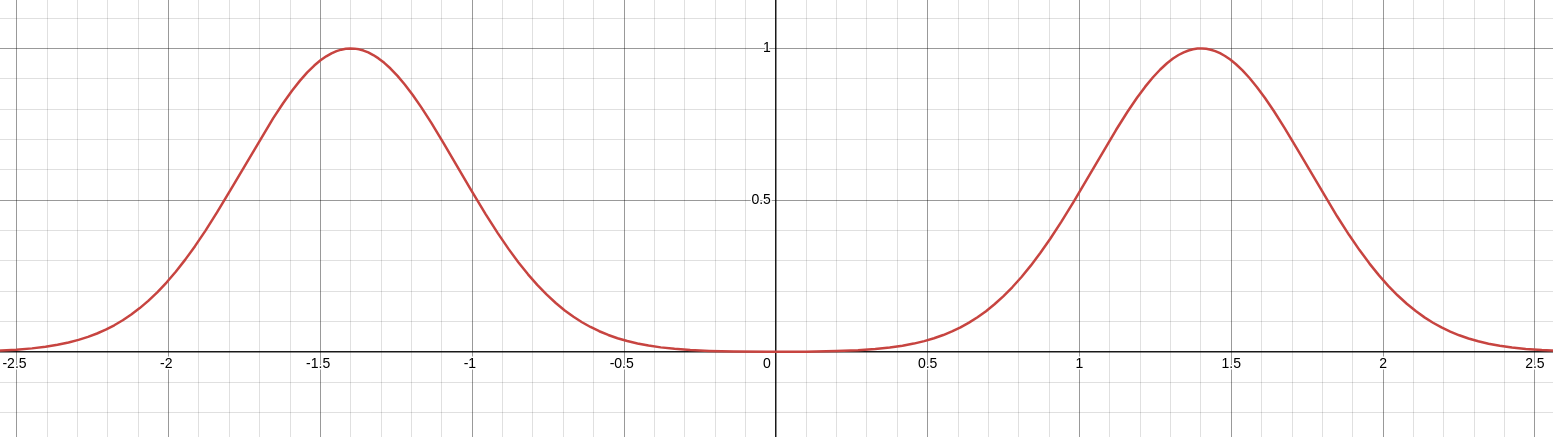
\includegraphics[width=0.9\textwidth]{fig/densi_spec_sym}
	\caption{Exemple de densité spectrale d'un signal réel ESP A 1,4}
	\label{fig:densi_spec_sym}
\end{figure}
\\
Même problème avec la covariance qui sera toujours nulle pour les signaux réels. De là en conclure que la fréquence instantanée de n'importe quel signal réel est toujours décorrélée du temps serait, pour le moins, insatisfaisant.
\\

Pour résoudre ces problèmes, il suffirait de ne conserver que la partie positive du spectre du signal. On s'intéresserait alors au signal transformée $\SA{x}$ tel que :
\[\mathcal{F}\big[\SA{x}\big] = 2\one_{\R^+}\fou{x}\]
où $\one_E$ est la fonction indicatrice sur l'ensemble $E$ et où le facteur 2 permet de conserver l'énergie du signal.
Avec la transformée de Fourier inverse, ce nouveau signal s'écrit alors :
\[\SA{x} = \mathcal{F}^{-1}\big[ 2\one_{\R^+}\fou{x} \big] = 2 \mathcal{F}^{-1}\big[\one_{\R^+}\big] * x\]
La transformée inverse de cette indicatrice (qui n'est autre que la fonction de Heavyside) n'est pas définie au sens classique, mais l'est au sens des distributions. Pour l'écrire, on introduit la distribution suivante :


\begin{definition}[valeur principale de Cauchy]\label{def:vp&Hilb}
	On appelle \emph{valeur principale de Cauchy} la distribution, notée $\vpC$, telle que :
	\begin{equation}
		\begin{aligned}
			\forall \varphi\in\mathcal{S}(\R),\qquad 
			\left\langle \vpC, \varphi \right\rangle 
			= \fint_0^t \frac{\varphi(t)}{t}dt 
			&\defeq \lim_{\varepsilon\lr0^+} \int_{-\infty}^{-\varepsilon} \frac{\varphi(t)}{t}dt + \int_{+\varepsilon}^{+\infty} \frac{\varphi(t)}{t}dt \\
			&= \int_0^{+\infty} \frac{\varphi(t) - \varphi(-t)}{t}dt
		\end{aligned}
	\end{equation}
	Ici $\mathcal{S}(\R)$ est l’espace de Schwartz des fonctions $C^\infty$ à décroissance rapide et la limite en $\varepsilon$ assure que l'intégrale (impropre) converge bien. Sa valeur est également appelée \emph{valeur principale} de l'intégrale. 
\end{definition}

La distribution vp$\frac{1}{x}$ est la valeur principale de la fonction inverse dans le sens où son produit avec l'identité donne 1 $\big(\left\langle id_\R \times \vpC, \varphi \right\rangle = \left\langle \vpC, id_\R \times\varphi \right\rangle=1\big)$ mais avec des propriétés d'intégration supplémentaires. Entre autre :


\begin{propriete}\label{prop:fou2vp}
	La transformée de Fourier de la valeur principale de Cauchy est donnée, au sens des distributions, par :
	\begin{equation}
		\mathcal{F} \left[\vpC \right]= -i \pi\, \sign{} 
	\end{equation}
	On en déduit la transformée de Fourier inverse :
	\begin{equation}
		\mathcal{F}^{-1}\big[ 2\one_{\R^+} \big] = \mathcal{F}^{-1}\big[ 1 + \sign \big] = \delta + \frac{i}{\pi} \vpC
	\end{equation}
\end{propriete}


\begin{demo}
	juste pour le plaisir. Par définition, la transformée de Fourier de la valeur principale est telle que,\\ $\forall \varphi\in\mathcal{S}(\R)$ :
	\begin{align*}
		\left\langle \mathcal{F} \left(\vpC \right), \varphi \right\rangle = \left\langle \vpC, \hat{\varphi} \right\rangle 
		&= \fint_\R \frac{\hat{\varphi}(\nu)}{\nu} d\nu \\
		&= \int_0^{+\infty} \frac{\hat{\varphi}(\nu) - \hat{\varphi}(-\nu)}{\nu} d\nu \\
		&= \int_0^{+\infty} \frac{1}{\nu} \left( \int_\R\varphi(t)e^{-2i\pi \nu t}dt - \int_\R\varphi(t)e^{2i\pi \nu t}dt \right)d\nu \\
		&= \int_0^{+\infty} \frac{1}{\nu}\int_\R\varphi(t)\big(e^{-2i\pi \nu t} - e^{2i\pi \nu t}\big)dt\, d\nu \\
		&= \int_0^{+\infty} \frac{1}{\nu}\int_\R-2i\varphi(t)\sin(2\pi \nu t)dt\, d\nu \\
		&= -2i\int_\R\varphi(t)\int_0^{+\infty} \frac{\sin(2\pi \nu t)}{\nu}d\nu\, dt
	\end{align*}
	En posant $u=2\pi\nu t\sign(t)$ (le signe de $t$ assure que l'on ait le même signe dans et hors du sin), on obtient :
	\begin{align*}
		\left\langle \mathcal{F} \left[\vpC \right], \varphi \right\rangle &= -2i\int_\R\varphi(t)\int_0^{+\infty} \sign(t)\frac{\sin(u)}{u}du\, dt \\
		&= -2i\int_\R\varphi(t)\frac{\pi}{2}\sign(t), dt \\
		&= \big\langle -i\pi\sign, \varphi \big\rangle
	\end{align*}
\end{demo}

\begin{definition}[Transformée en SA et de Hilbert]\label{def:transfo_sa&hilbert}
	On définie alors la \emph{transformée en signal analytique} (SA) de tout signal $x$ par l'application :
	\begin{equation}\label{eq:transfo_SA}
		\SA{x} = \sa{x} \defeq 2 x*\mathcal{F}^{-1}\big[\one_{\R^+}\big] :\ \begin{aligned} 
			\R \quad &\lr\qquad\quad \C \\	
			t\quad &\longmapsto\ x(t) + \frac{i}{\pi}\fint_\R \frac{x(s)}{t-s}ds
		\end{aligned}
	\end{equation}
	Par construction, on a bien $\mathcal{F}\big[\SA{x}\big] = 2\one_{\R^+}\fou{x}$, et on dira plus généralement de tout signal dont le spectre est réel positif que c'est un \emph{signal analytique}.
	\\
	L'intégral à droite de \eqref{eq:transfo_SA} est appelle \emph{transformée de Hilbert} du signal. Elle est notée :
	\begin{equation}\label{eq:transfo_Hilb}
		\mathcal{H}[x] :\ \begin{aligned} 
			\R \quad &\lr\qquad\quad \C \\	
			t\quad &\longmapsto\ \frac{1}{\pi}\fint_\R \frac{x(s)}{t-s}ds =  \frac{1}{\pi}\left(\vpC\right)*x
		\end{aligned}
	\end{equation}
\end{definition}

Par souci de commodité, plutôt que redéfinir tout le vocabulaire développé plus haut (fréquence moyenne, temps moyen, \etc) pour les signaux réel via la transformation $\mathcal{A}$, dans la suite du mémoire on travaillera directement avec $\SA{x}$. %^(et on verra que c'est essentiel).




\subsubsection{Interprétabilité des signaux analytiques}\label{subsec:Bedrisan&AM-FM}


Dans les cas des signaux réels, la transformée de Hilbert est à valeur dans $\R$. Aussi, la transformée $\SA{x}$ à pour partie réelle $x$ et pour partie imaginaire $\mathcal{H}[x]$. Sous forme exponentielle, cela donne :
\[\SA{x}(t) = a(t)e^{i\phi(t)}\quad \Lr\quad \left\{\begin{aligned}x(t) &= a(t) \cos\phi(t) \\\mathcal{H}[x](t) &= a(t) \sin\phi(t)
\end{aligned}\right.\]
On obtient alors on décomposition de $x$ en une paire $(a,\phi)$ telle que discuté plus haut.

\begin{definition}[Amplitude et phase instantanée]\label{def:ampli&phase_instant}
	On définie ainsi l'\emph{amplitude instantanée} $a_x$ et la \emph{phase instantanée} $\phi_x$  de tout signal $x$ comme étant respectivement l'amplitude et la phase de $\SA{x}$ :
	\begin{align}\label{eq:ampli&phase_cano}
		a_x &= \big|\SA{x}\big|   &   \phi_x &= \arg\big(\SA{x}\big)
	\end{align}
\end{definition}

\begin{remarque}
	Il est important de noter que si un signal est présenté sous la forme  $\ x=a\cos\phi$, rien n'implique que $a$ et $\phi$ corresponde à l'amplitude et la phase instantanée du signal. Si ce n'est pas le cas, c'est que cette décomposition n'était ``pas la bonne'' en cela qu'elles ne s’interprètent pas comme l'on aimerait.
\end{remarque}

Pour comprendre comment cette transformation ``sélectionne'' la fréquence instantanée, détaillons le cas où $x$ s'écrit comme produit de deux signaux pures (\cref{fig:exemple_tSA_1/2}) :
\[x(t) = \cos (2\pi\nu_1t)\cos (2\pi\nu_2t)\]
\\
On montre sans mal\footnote{\itshape
	$\fou{x}$ est donné par 4 Diracs, en ne gardant que ce non nul sur $\R^+$ on obtient le spectre de $\SA{x}$ et il reste plus qu'à inverser la transformée de Fourier.}
que si $\nu_1\geq\nu_2$, alors la transformée en SA de $x$ s'écrit :
\[\SA{x} = \cos \left(2\pi\nu_2 t\right) e^{2\i\pi\nu_1 t}\]

\begin{figure}[h]\centering
	%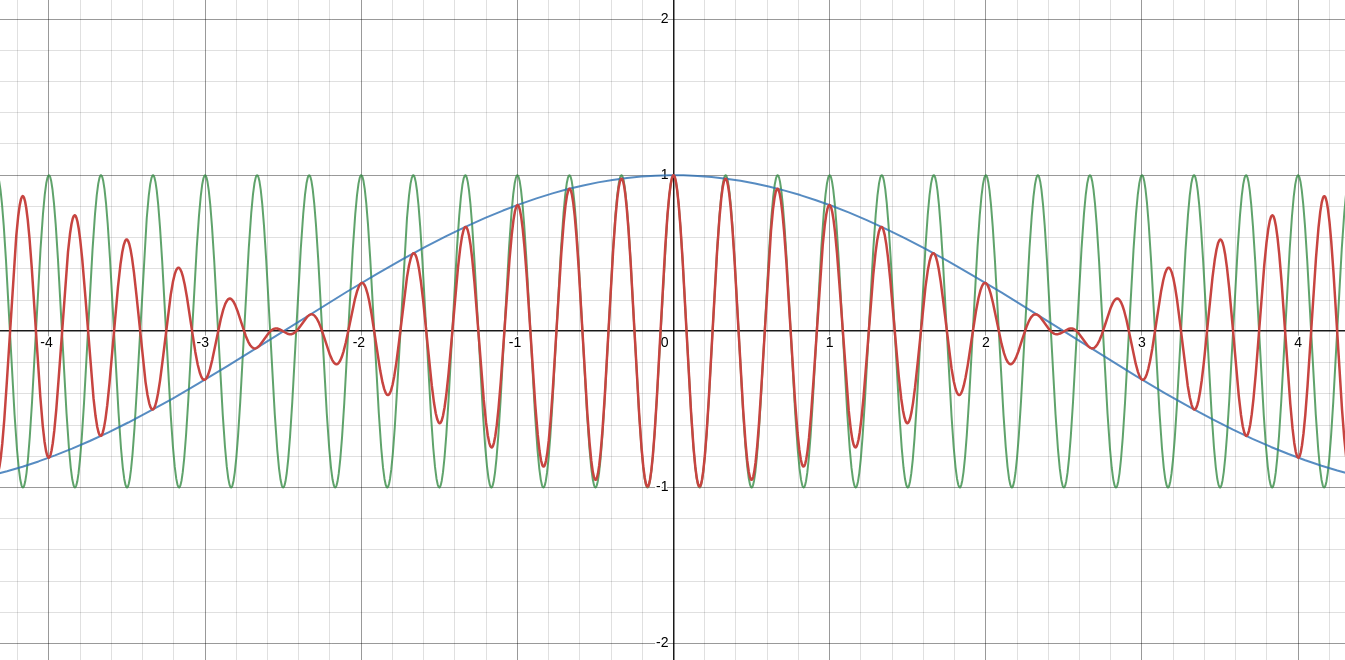
\includegraphics[width=0.48\textwidth]{fig/ex SA - 11.png}\hfill
	%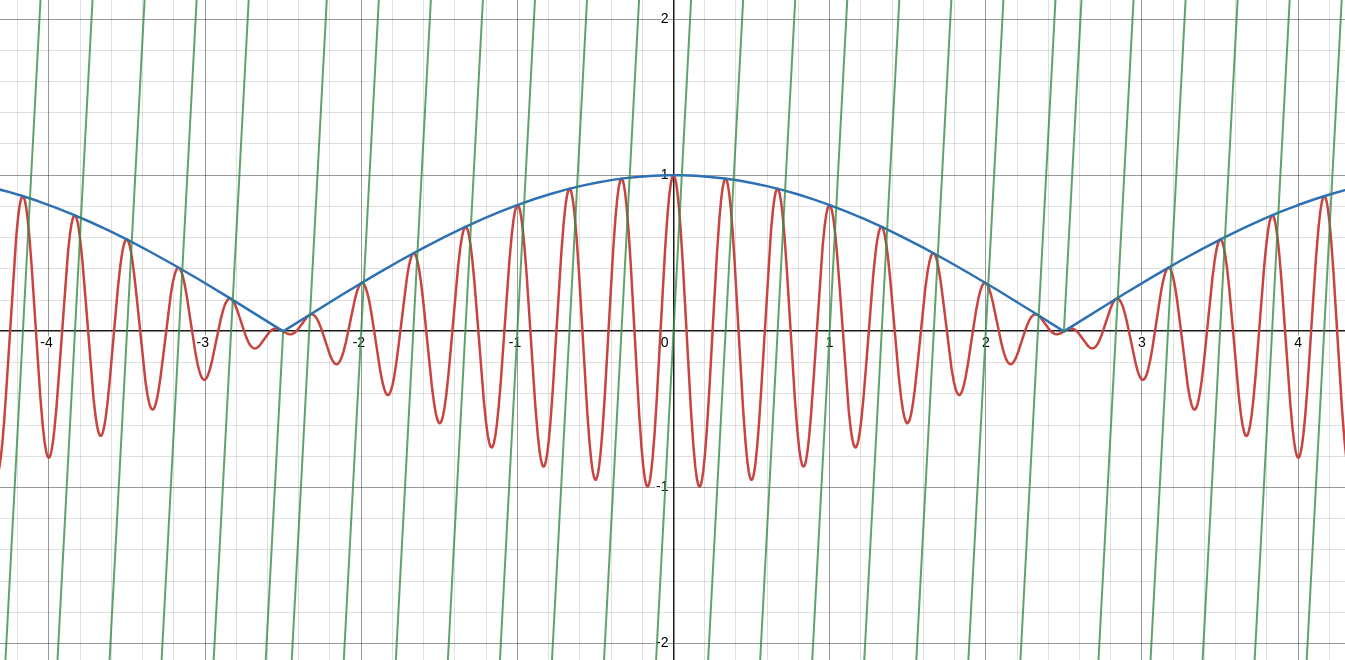
\includegraphics[width=0.48\textwidth]{fig/ex SA - 12.png}
	\caption{Représentation graphique du signal $x$ (rouge) avec $\nu_1=3$ et $\nu_2=0.1$. Sur l'image de gauche, avec signaux de fréquences pures (bleu et vert). Sur l'image de droite, avec son amplitude (bleu) et sa phase instantanée (vert). Les discontinuités de la phase sont dû à l'arrondi à $2\pi$  près de l'argument de $\SA{x}$ et à la façon dont il est calculé lorsque le signal s'annule (mise à 0). Voir \href{https://www.desmos.com/calculator/gcedcdfkhr}{ici} pour un graphique dynamique.}
	\label{fig:exemple_tSA_1/2}
\end{figure}
\noindent
Le signal $\SA{x}$ n'est ici pas sous forme exponentielle à proprement parler puisque le cosinus peut être négatif (pour s'y ramener, il suffit de passer le cos en valeur absolue et d'ajouter $\pi$ à l'argument lorsque nécessaire) mais l’avantage de cette forme est qu'elle fait clairement apparaître les fréquences $\nu_{1,2}$. En particulier, la fréquence instantanée du signal est la plus grandes des deux fréquences $\nu_1$ et $\nu_2$. La plus petite, elle, se retrouve dans l'amplitude. 
\\
Ce résultat est rassurant en cela qu'il est plus naturel de voir le cosinus de basse fréquence comme modulant celui de haute fréquence que l'inverse comme on le voit sur la première image de la figure \ref{fig:exemple_tSA_1/2}. 
\\
Aussi, en mettant les hautes fréquences du signal dans la fréquence instantanée, on s'assure de limiter les variations de l'amplitude. Cela apporte bien plus de contrainte en terme de décomposition $(a_x,\phi_x)$, en cela qui si l'inverse étant vrai, alors toute les fréquences pourrait être envoyé dans l'amplitude, ce qui laisserait la phase invariante.
\\

Cela étant dit, lorsque l'on fait varier $\nu_1$ et $\nu_2$, le résultat n'est pas toujours si intuitif. C'est notamment le cas lorsque les deux deviennent de plus en plus proche :

\begin{figure}[h]\centering
	%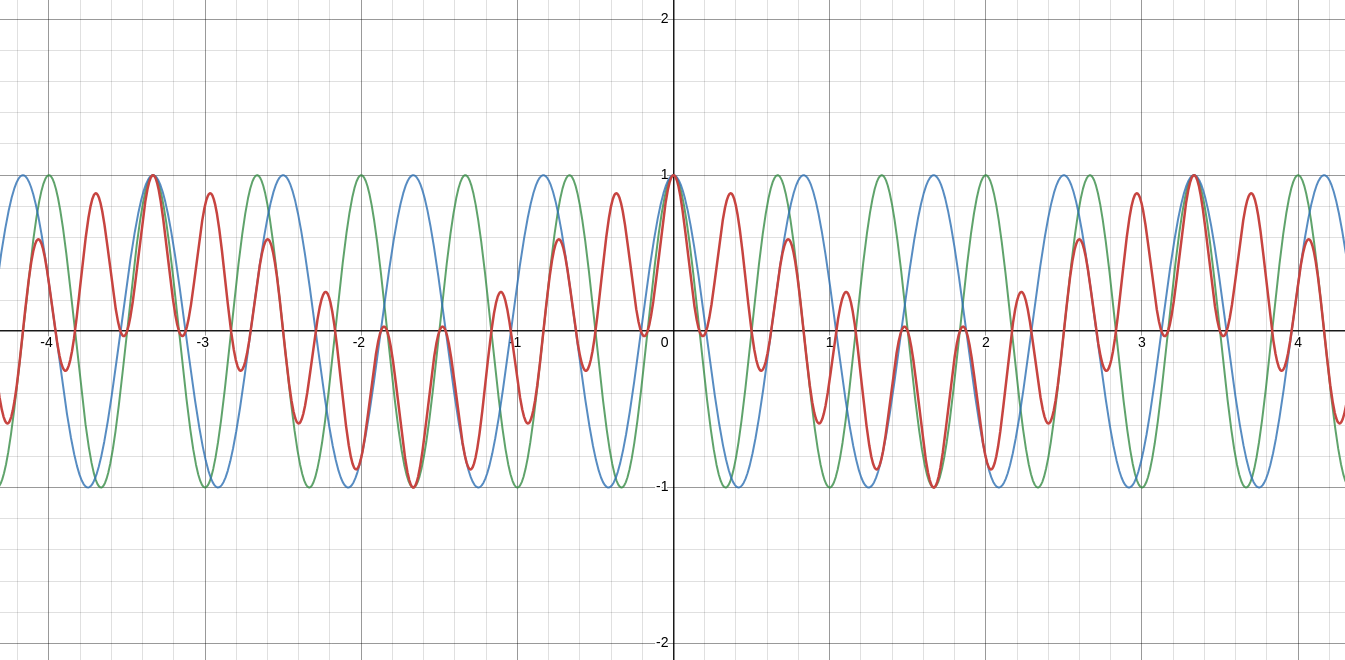
\includegraphics[width=0.48\textwidth]{fig/ex SA - 21.png}\hfill
	%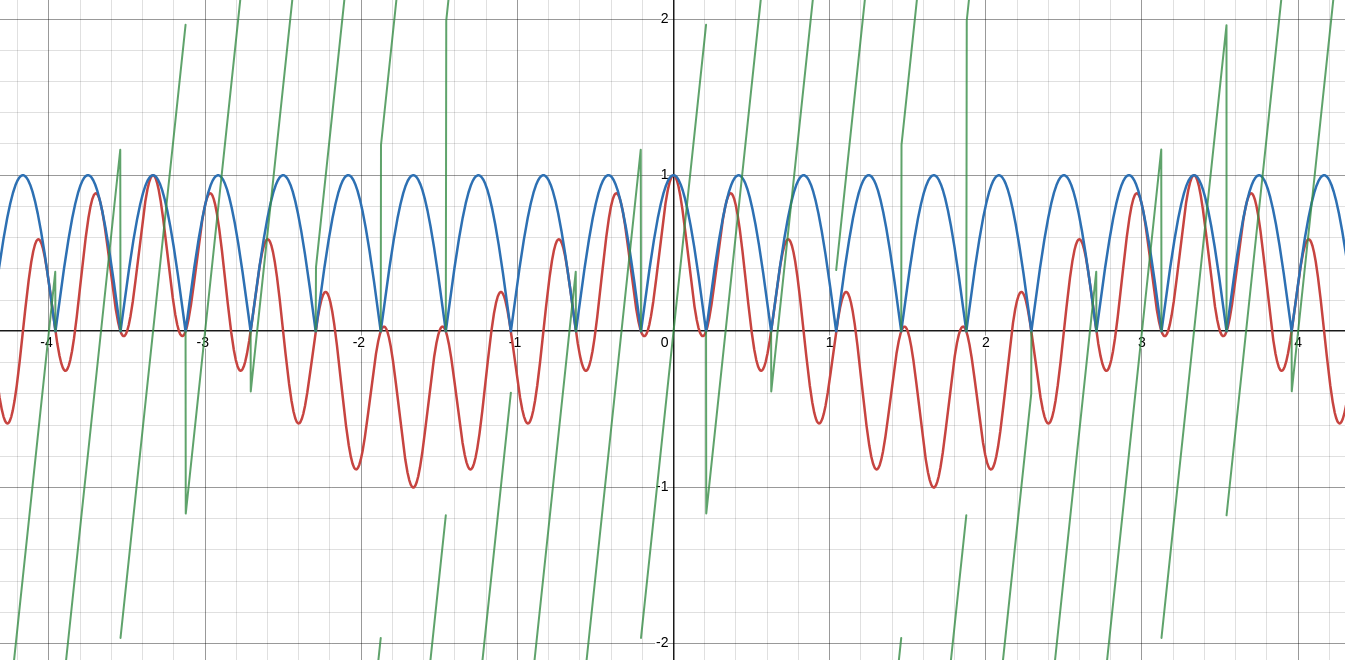
\includegraphics[width=0.48\textwidth]{fig/ex SA - 22.png}
	\caption{Idem que pour la figure \ref{fig:exemple_tSA_1/2} précédente, avec cette fois $\nu_1=1.5$ et $\nu_2=1.3$.}
	\label{fig:exemple_tSA_2/2}
\end{figure}

Pour comprendre pourquoi l'amplitude ne fait pas ce qu'on attendrait d'elle, on introduit le théorème de Bedrosian :

\begin{theoreme}[de Bedrosian]\label{theo:2Bedrosian}
	Dans sa formulation la plus générale, le théorème de Bedrosian énonce que donnée si deux fonctions $f,g\in L^2(\R)$ sont telles l'une des trois assertions suivantes est vraie :
	\newline
	\begin{itemize}%[label=\textit{\arabic*}. ]
		
		\item $\exists \lambda\in\R^+\ |\ \supp \fou{f} \subset [-\lambda, +\infty[,\ \supp \fou{g} \subset [\lambda, +\infty[$\label{item:1condi_theo2Bedrosian}
		
		\item $\exists \lambda\in\R^+\ |\ \supp \fou{f} \subset ]-\infty, \lambda],\ \supp \fou{g} \subset ]-\infty,-\lambda]$ \label{item:2condi_theo2Bedrosian}
		
		\item $\exists (\lambda_1,\lambda_2)\in \R^+\times\R^+ \setminus\{(0,0)\}\ |\ \supp \fou{f} \subset [-\lambda_1, \lambda_2],\ \supp \fou{g} \subset \R\setminus[-\lambda_2,\lambda_1]$
		
	\end{itemize}
	alors la transformée de Hilbert de leur produit est donnée par la formule (voir \cite{wang_simple_2009} pour une démonstration) :
	\begin{equation}\label{eq:2Bedrosian}
		\hilb{fg} = f\hilb{g}
	\end{equation}
\end{theoreme}

Dans le cas d'un signal réel, suivant la \cref{def:ampli&phase_instant} on peut écrire $\ x=a_x\cos\circ\phi_x$.
Comme $a_x$ et $\phi_x$ sont réelles, seule la deuxième condition du théorème de Bedrosian peut être satisfaite pour peu que $\lambda_1=\lambda_2$. Ainsi :

\begin{corollaire}\label{coro:AM-FM}
	Toujours avec les même notations, si $a_x\in L^2(\R)$, $\cos\phi_x\in L^2(\R)$ et qu'il existe $\lambda\in\R^{+_*}$ tel que :
	\[\supp \Fou{a_x} \subset [-\lambda, \lambda],\quad \supp \Fou{\cos\phi_x} \subset \R\setminus[-\lambda,\lambda]\]
	Alors on a :
	\begin{align*}
		\hilb{x} &= a_x\hilb{\cos \phi_x}  &  \qquad\qquad&\text{et si }a_x(t)\neq 0,  &  \hilb{\cos \phi_x}(t) = \sin\phi_x(t)
	\end{align*}
\end{corollaire}

Dans ce cas, 


\newpage

\bibliography{ref.bib}{}
\bibliographystyle{siam}

\end{document}